%second chapter of your thesis
\chapter{Hardware}
Onze robot werkt met behulp van 3 zelfgemaakte PCB's. Twee ervan zijn de combinatie van de Motorshield en de Arduino/Atmega en de andere is een printplaat om de bekabeling te reduceren.





\section{Tussenstuk}
Het tussenstuk is een PCB waarop alle lijnen van de infra rood sensoren toekomen en worden doorgegeven aan de AtMega. Het voordeel van deze printplaat is dat we nu slechts 1 GND en 1 VCC lijn moeten voorzien tussen het printplaatje en de Arduino. We hebben op dit printplaatje ook de mogelijkheid voorzien om de Bluetooth-module en de RFID-reader aan te sluiten. Nadien hebben we ontdekt dat de RFID-reader niet kon worden aangesloten op onze hoofd Arduino waardoor we de RFID-reader ook niet verbonden met dit tussenstuk maar wel rechtstreeks aan de hulp-Arduino. Verbinden met het tussenstuk zou de vereenvoudiging van de bekabeling teniet doen. Het probleem omtrent de RFID-reader leggen we later nog uitgebreider uit. 






We hebben dus 10 5V-aansluitingen voorzien, 10 GND-aansluitingen, 6 aansluitingen voor de outputsignalen van de sensoren en de pinnen die nodig zijn voor de Bluetooth-module (Key, Vcc, GND, TXD, RXD en State). Niet alle zes de uitgangen van de Bluetooth-module moeten worden doorgestuurd naar onze Atmega, deze vereenvoudiging vindt ook plaats op deze PCB. Enkel de signalen Vcc, GND, TXD en RXD worden van een uitgang voorzien. Deze uitgangen worden dus doorverbonden met de Atmega. De Vcc en de GND aan deze uitgang zorgen dus ook voor de voeding van de volledige PCB. We maken gebruik van de HC-05 Bluetooth-module, een foto van de module wordt weergegeven in afbeelding~\ref{fig:HC05}.
\newpage
\begin{figure}[h]
\centering
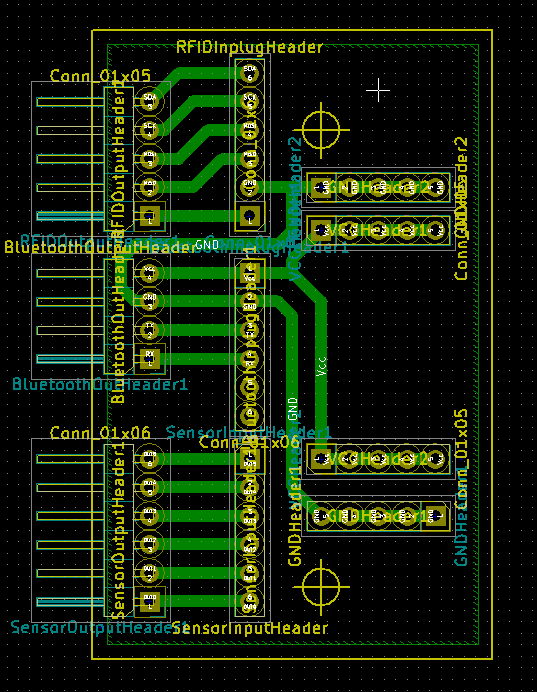
\includegraphics[width=0.3\textwidth]{tussenstukPCB.png}
\caption{Routing van de PCB die als verlengstuk dient. \label{tussenstukPCB}}
\end{figure}


\begin{figure}[h]
\centering
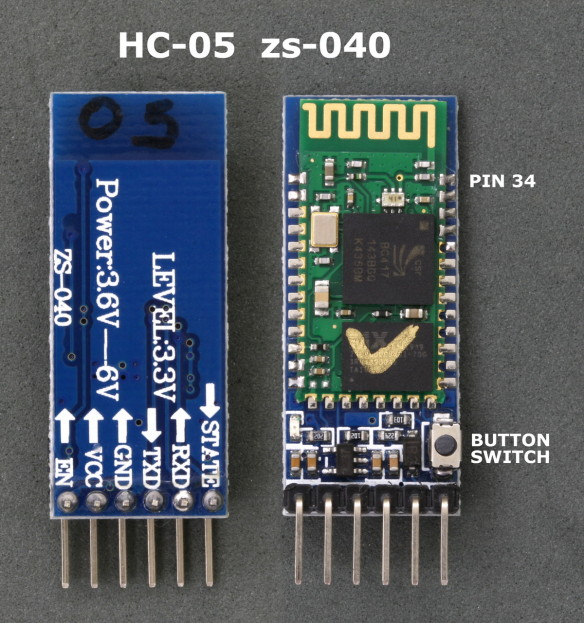
\includegraphics[width=0.3\textwidth]{HC05.jpg}
\caption{De gebruikte Bluetooth-module, ingeplugd op de verlengPCB.}
\label{fig:HC05}
\end{figure}
\section{Ardumoto}
\subsection{Ardumoto RFID}
De tweede printplaat die we ontworpen hebben, is eigenlijk de combinatie van de Atmega en de Motorshield, hoewel we hier enkel gebruik zullen maken van de Atmega en de L298 zullen laten voor wat het is. Deze PCB zorgt voor de aansturing en uitlezing van de RFID-reader. We hebben een tweede Atmega nodig omdat de RFID-reader volgende signalen nodig heeft om correct aangestuurd te worden: SS/RX, SCK, MOSI, MISO/TX, IRQ, GND, RST, Vcc. 3 van deze pinnen worden ook gebruikt voor de motoraansturing. SCK is namelijk dezelfde pin als die voor de aansturing van de richting van motor B. MOSI is dezelfde pin als die voor de aansturing van de snelheid van motor B. En de laatste overeenkomstige pin is die van MISO, dit is namelijk dezelfde pin als de aansturing van de richting van motor A. Deze pinnen kunnen geen twee signalen gelijktijdig verwerken waardoor we dus opteerden om gebruik te maken van de hulp-Arduino. Een andere mogelijkheid om dit probleem op te lossen kon erin bestaan om gebruik te maken van een RFID-reader die het $I^{2}C$ principe hanteert, in plaats van ISP. Door $I^{2}C$ te gebruiken zouden we geen conflicten met de pinnen gehad hebben en zouden we dus ook geen tweede PCB nodig gehad hebben. We maken gebruik van de RFID-reader-module, namelijk de MRFC522, dewelke wordt weergegeven in figuur~\ref{fig:MRFC522}. Om een RFID-tag zo goed mogelijk uit te lezen moet de reader op $\approx$ 1 cm boven de tag passeren. We hebben hiervoor zelf een RFID-houdertje geprint met de 3D-printer zodat deze afstand ten alle tijden constant blijft.
\begin{figure}[h]
\centering
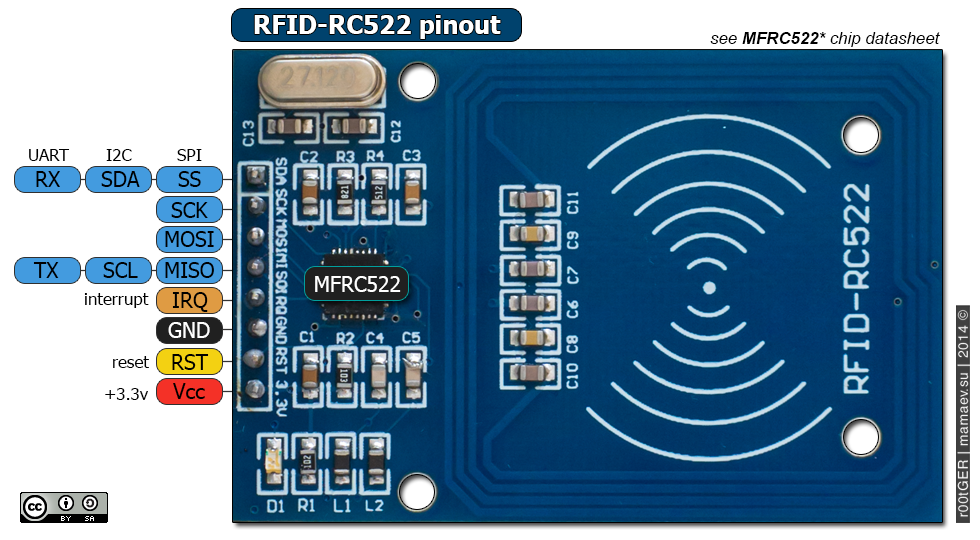
\includegraphics[width=0.75\textwidth]{MRFC522.png}
\caption{Gebruikte RFID-reader MRFC522. \label{fig:MRFC522}}
\label{fig:ACEquiv}
\end{figure}
\subsection{Ardumoto Motor}
Deze PCB is verantwoordelijk voor de aansturing van de motoren en ook voor het doorsturen van de signalen naar de Raspberry Pi via de HC-05. Na het finaliseren van de PCB bleken er nog enkele fouten te zijn geslopen in onze versie. Enkele footprints waren aan de kleine kant waardoor sommige componenten slechts heel nipt op de koper-eilandjes pasten. Na ons prototype hadden we deze fout aangepast maar bleek onze correctie nog onvoldoende te zijn om comfortabel te kunnen solderen. Ook een condensator bleek bij het testen niet goed vastgesoldeerd te zijn waardoor we slecht contact kregen wat we opgelost hebben met een externe verbinding. Maar de grootste fout waarop we gestoten zijn, was dat een ingang van de L298 (de IC verantwoordelijk voor de motoraansturing) niet verbonden was met het PWRIN signaal waardoor er geen vermogen naar de motoren gestuurd werd. Dit kwam omdat er een hi\"erarchical label ontbrak in ons schema op de betreffende locatie aan de L298. We hebben dit probleem kunnen oplossen door een extra kabel te solderen van het PWRIN signaal naar de betreffende pin van de L298. \\
Als vertrekpunt van ons ontwerp zijn we vertrokken van het schema van een een Arduino Uno dat we op het internet konden downloaden. Als eerste konden we de USB interface voor de aansluiting van een USB-kabel weglaten aangezien we dit in ons finaal ontwerp niet nodig hadden. Voor het uploaden van een programma maken we dan gebruik van de ICSP-pinnen die we nauwkeurig verbinden met een andere Arduino die de code doorstuurt.  Alle LED's die normaal gezien aanwezig zijn op de Arduino Uno hebben we  weggelaten omdat we dit niet echt nodig hebben en dit onze arduino groter zou maken dan nodig. Om het het ons eenvoudiger te maken, pasten we in het schema ook de namen van de labels aan naar meer betekenisvollere namen zodat we de namen van de lijnen zo eenvoudiger konden interpreteren. Zo veranderden we bijvoorbeeld MISO door DIR A aangezien deze lijn verantwoordelijk was voor de richting van Motor A. (FOTO ATMEGA) R8 hebben we ook weggelaten aangezien dit een weerstandswaarde van 0 $\Omega$ heeft. Deze weerstand wordt voornamelijk gebruikt om een brugje te cre\"eren om er baantjes onder te kunnen trekken. Pinnen 27 en 28 hebben we niet nodig, dus mogen we de condensator hier rond ook verwijderen. De jumper hebben we weggelaten omdat we die niet nodig achtten. Eenmaal we het schema hadden die we nodig hadden was het tijd om te routen. We zijn er in geslaagd om een PCB te maken met afmetingen (52,324mm x 61.468mm). We konden dus ook strikt genomen onze printplaat deze afmetingen geven maar we hebben er bewust voor gekozen om de printplaat wat groter te maken, nl.  53.34mm x 73.152mm. We hebben hiervoor geopteerd omdat we dan bevestigingsgaten konden voorzien die passen in de voorziene gaten op de auto. We hebben begonnen met baantjes van 10 mills(= 0.254mm). En daarna hebben we zoveel mogelijk de baantjes verbreed tot maximaal 30 mills. Op de plaatsen waar het kon hebben we daarvoor ook de baantjes verlegd, zodat we ze breder konden maken. We hebben de vias ook op een grotere maat gezet, alle afmetingen worden grafisch weergegeven in de tabel.\\
\begin{center}
	\begin{tabular}{ | l | l | l | l | l |}
	\hline
	  & Clearance & Track Width & Via Dia & Via Drill\\ \hline
	Default & 0.25 & 0.25 & 0.6 & 0.4\\ \hline
	0.5 & 0.25 & 0.5 & 0.7 & 0.5 \\ \hline
	12 mills & 0.25 & 0.3 & 0.6 & 0.4 \\ \hline
	15 mills & 0.25 & 0.38 & 0.6 & 0.4 \\ \hline
	30 mills & 0.25 & 1 & 0.6 & 0.4 \\ \hline
	\end{tabular}
\end{center}
We hebben ook de 12 mills erbij gezet omdat deze dikte van de baantjes dan exact gelijk is aan de breedte van de bevestigingspinnen van een SMD-component. Enkele baantjes zijn ook ingesteld op 15 mills. We hebben natuurlijk ook geprobeerd het aantal vias te beperken, wat ons wel redelijk goed gelukt is, we hebben er slechts 20 gebruikt. We merkten dat bij onze eerste pogingen om de printplaten te drukken de fijnste baantjes vaak volledig opgelost waren door te lang in het zuurbad te liggen. We kregen de tip om gebruik te maken van een opgevuld vlak, met als reden dat we nu veel minder lang de PCB in het zuurbad moesten steken want er moest veel minder koper opgelost worden. Achteraf gezien konden we eigenlijk aan de beide vlakken een functie geven bv. GND-vlak, wij hebben dit geen betekenis gegeven. Eens de PCB volledig bestukt was, wilden we het eerst testen met een standaardprogramma voor de atmega nl. Getting To Blinky. Dit werkte direct en daarom veronderstelden we verkeerdelijk ook direct dat de volledige PCB werkzaam was. We bespreken dit uitgebreid in het hoofdstuk~\ref{Moeilijkheden}. 

%In het vorig hoofdstuk hebben we naar deze tekst verwezen\label{verwijzing}.
